In this chapter, detailed description of NF chaining mechanism in kernel space is given. 
The architecture makes use of existing Netfilter in Linux. First, the role of Netfilter system in the network stack is explained. Second, the main structure of Kernel-based NFCI is described in chapter 4.2. It consists of identification of flows and NF chaining mechanism. 

\subsection{Netfilter: Overview}
Netfilter is a software inside the Linux 2.4.x and later kernel series, which enables packet filtering and packet mangling. It is a set of hooks that are placed in several stages in network stack and in each hook multiple kernel modules can be registered. Each of the kernel module will work as a NF, such as Firewall and NAPT. 
Figure \ref{fig: netfilter_system} shows the network stack and five netfilter hooks embedded inside it. The bottom is the device driver and the more it goes up the network layer does as well to reach the transport protocol (Layer 4). As packets progress through the stack, the registered kernel modules in the hook will be triggered. 
The following hooks are located in meaningful positions in the stack:
\begin{itemize}
	\item PRE\_ROUTING : This hook is triggered by incoming packet soon after entering the network stack. This is processed before the packet reaches the routing subsystem.
	\item LOCAL\_IN : This hook is processed after the packet has been routed and is destined to the local host.
	\item FORWARD : This hook is processed after the packet has been routed and is to be forwarded to another host. 
	\item LOCAL\_OUT : This hook is triggered by locally created packet as soon as it enters the stack.
	\item POST\_ROUTING : This is the last hook that the outgoing or transmitted packet passes before being put out on the wire. 
\end{itemize}

\begin{figure*}
	\centering
	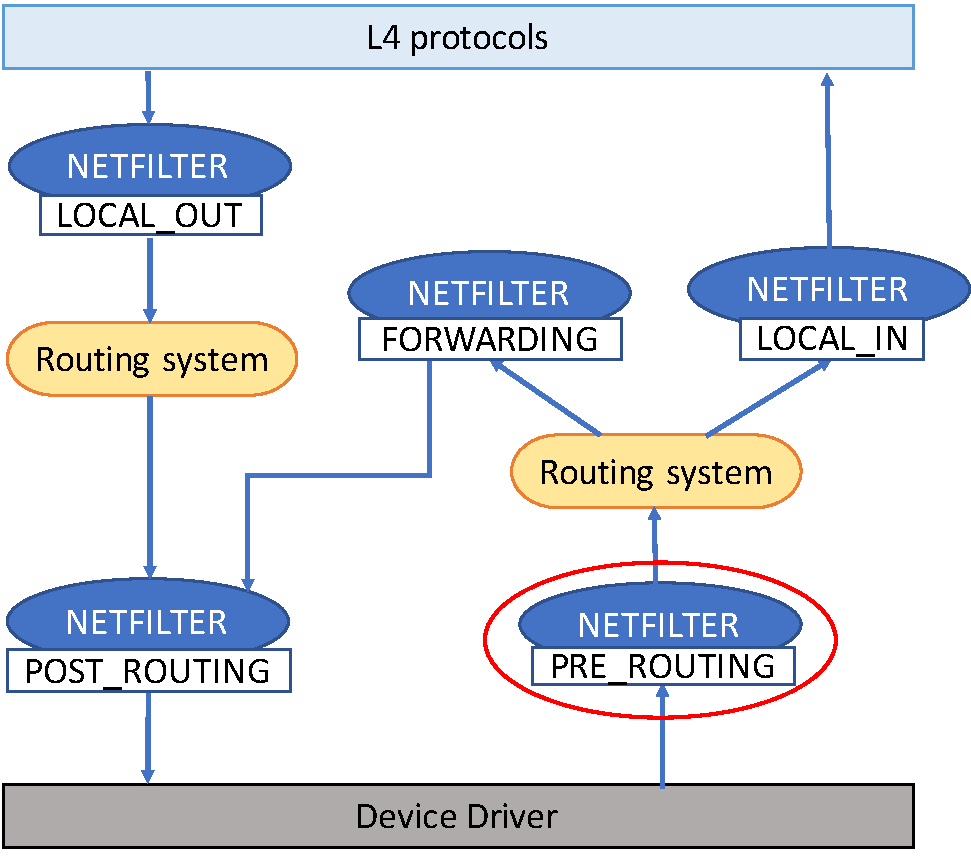
\includegraphics[width=90mm]{pics/netfilter_system.pdf}
	\caption{Netfilter hooks in network stack}
	\label{fig: netfilter_system}
\end{figure*}

Kernel modules that are registered in a hook according to the its priority. The lower the priority value is, the earlier it gets executed. Each kernel module will return a verdict indicating the result of the process. 

\subsection{Netfilter: Table}
Netfilter supports Firewall, NAPT and so on. Each of these NF has its own "Table" to organize the rules. Rule is used to specify which kind of flow is targeted for the specific action, such as filtering in case of Firewall. In each netfilter hook, the following tables can be registered. 


\begin{table}[tb]
	\centering
	\caption{List of tables in Netfilter hooks}	
	\begin{tabular}{|c|c|c|c|c|c|}
		\hline
		\backslashbox{Tables}{Hooks} & 	PREROUING & INPUT & FORWARD & OUTPUT & POSTROUTING \\
		\hline
		\hline
		Mangle & $\bigcirc$ & $\bigcirc$ & $\bigcirc$ & $\bigcirc$ & $\bigcirc$ \\
		\hline
		CT & $\bigcirc$ & & & $\bigcirc$ & \\
		\hline
		DNAT & $\bigcirc$ & & & $\bigcirc$ & \\
		\hline
		Filter & & $\bigcirc$ & $\bigcirc$ & $\bigcirc$ & \\
		\hline
		SNAT & & $\bigcirc$ & & & $\bigcirc$ \\
		\hline
	\end{tabular}
\end{table}

\begin{itemize}
	\item Mangle Table : Mangle Table is used to alter the IP headers of the packet in various ways. For instance, one can adjust the TTL value of a packet to either lengthen or shorten the number of network hops. 
	\item Connection Tracking Table (CT) : CT enables stateful operation by associating packets with a connection. CT checks each packet against existing connections. If the first packet of a new flow enters the system, a new connection will be created. Otherwise the state of the connection will be updated accordingly. Only CT can be used, for example allowing only packets that are associated with an established connection. It is also common to use CT with NFs that want to see the packets in the context of an ongoing connection. NAPT is one of the such NF that make use of CT.
	\item DNAT / SNAT Table : NAT is divided into two DNAT and SNAT. DNAT is responsible of changing the destination IP address or port, whereas SNAT changes source IP or port. DNAT table can be placed in PRE\_ROUINTG and OUTPUT hooks, both before the routing subsystem because the change of destination part would change the routing decision as well. Meanwhile SNAT takes place at LOCAL\_IN and POST\_ROUTING, both before being delivered to the destined host. 
	\item Filter Table : The filter table is used to make decision about whether to allow packet to continue to its destination or drop the packet. Unlike the above tables, when a rule matches only a verdict whether to accept or drop is returned without doing any specific process. This is normally used for Firewall for filtering mechanism. 
\end{itemize}
 


\subsection{Netfilter: Rule and Target}
In each table a sequence of rules are installed, which forms a "chain of rules". The rules will be evaluated from top to down in the chain. A rule is registered with a target component, which has function or verdict. Any target returns integer value named verdict which determines how the packet will be handled.
 The verdict value XT\_CONTINUE and XT\_RETURN are special. When the verdict is XT\_CONTINUE the next rule in the chain is further evaluated. And XT\_RETURN means to jump to another rule chain. The other main verdicts are NF\_ACCEPT, NF\_DROP. NF\_DROP tells to discard the packet. NF\_ACCEPT means that the traversal of rule chain terminates in the table and the packet will be further processed by the next table if any or return from the netfilter system to the network stack. 
 
There are following cases when a rule matches: 
\begin{enumerate}
\renewcommand{\labelenumi}{\arabic{enumi})}
	\item Only a verdict (NF\_ACCEPT, NF\_DROP, etc.) gets returned without doing any process.
	\item Registered function in the target is executed and returns verdict according to the result of the process.
	\item Jump to another rule of chain. 
\end{enumerate}

Figure \ref{fig: ip_chains} shows an abstract image of traversal of rule chain. 

Rule Chain0 and Rule Chain1 belong to the same table. Smaller boxes in the rule chains represents sets of rule and target. A packet will be evaluated from the top of rule chain until the target's verdict returns NF\_DROP or NF\_ACCEPT. Suppose we get a TCP packet with destination port X and destination IP y.y.y.y and we need to process it through firewall table in figure \ref{fig: ip_chains}. The packet enters rule chain0 for screening and first checked against "UDP port = Y" rule. Since the first rule doesn't match, it proceeds to the next rule "proto = TCP". The second rule matches and therefore the target is executed. The target is a verdict "XT\_RETURN" so the packet jumps to another chain, in this case Rule Chain1 for further screening. The first and second rule in rule chain 1 both don't match so the packet jumps back to the rule chain0 to start from the third rule. The third rule matches so the target  which is a function in a registered kernel module is executed. This function1 returns verdict and if the verdict is either NF\_DROP or NF\_ACCEPT, the screening in this table terminates. If the verdict is XT\_CONTINUE then it continues to the next rule. The last evaluated rule's target decides the verdict of the packet. 

\begin{figure*}
	\centering
	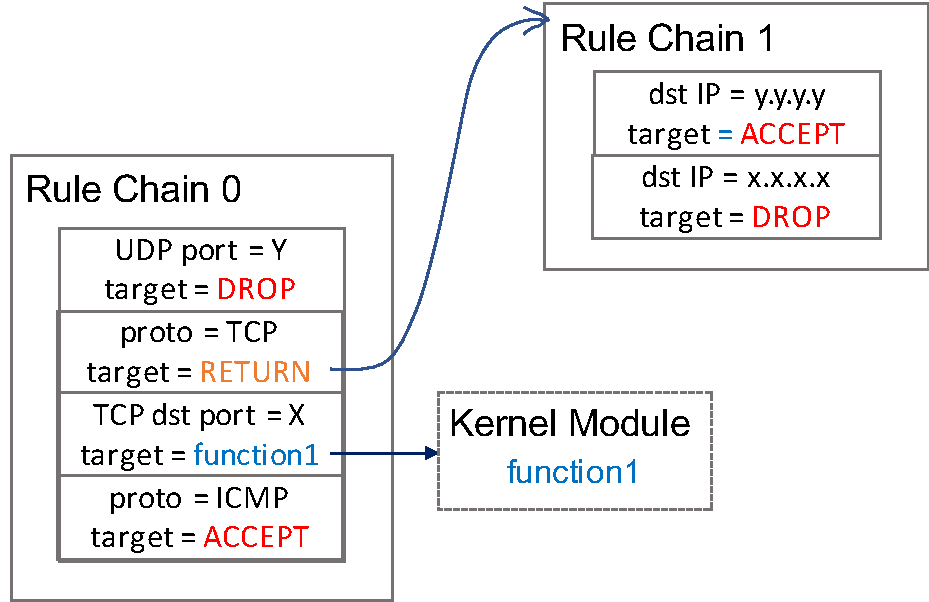
\includegraphics[width=90mm]{pics/ip_chains.pdf}
	\caption{Ipchains rules and targets}
	\label{fig: ip_chains}
\end{figure*}

\section{Kernel-based NFV architecture}
There are three main components in Kernel-based NFV. One is the identification of flow. The second is chaining of NFs, the system that enables packets to be processed by NFs in order. And the last is the NFs themselves. Any kind of NF consists of one kernel module or more. 

The NF chaining mechanism takes place in the PRE\_ROUTING hook which locates between hardware and routing subsystem in the network stack, which I call here "chaining point". 

\subsection{Network Function}
Any installed kernel modules exist in the same memory region as kernel so the functions in the modules can be seen from other modules and from kernel. This is why it is possible to call functions in kernel modules from network stack. Normally a NF consists of several kernel modules. And in this case, the very first function among kernel modules should be registered somewhere in the kernel and the subsequent functions in other kernel modules will be called in order. 

\subsection{Identification of flow}
In the kernel-based NFV host, sets of NF chain can be registered. When a network node participates in NF chaining, it is likely that many flows comes in and out. Not all the flows are to be processed by a single NF chain but only specific flows should pass its designated NF chains. So a mechanism is needed to specify which kind of flow should be treated by a chain of NF in the host. For example in OPNFV, OVS is used to direct flows to the right NFs which are VMs. OVS employs OpenFlow which can set a very detailed rules using vlan tag, incoming / outgoing port, etc. Kernel-based NFV distinguishes flows in granularity of 5-tuples. 5 tuples represent source / destination IP address, source / destination port number and the transport protocol. 

The identification of flow in 5-tuple is implemented using Filter table. As explained in chapter 4.1.2, Filter table carries out filtering by setting rule and verdict of NF\_DROP or NF\_ACCEPT. In stead of setting verdict in the target, pointer to the list head of chained NFs is registered. 

\subsection{Chaining of Network Functions}
I used Doubly Linked List (DLL) to implement NF chaining. DLL is a list that contains links to next and previous nodes. Unlike singly linked lists traversal is only one way, DLL allows traversal in both ways. 
Figure \ref{fig: dll} shows the framework of NF chain realized with DLL. DDL is chosen since adding and removing node can be done easily. A NF is represented by a node of gray box. A node is a nf\_target struct which has the following members: 
\begin{itemize}
	\item list\_head struct : list\_head struct has two pointers, next and prev, which respectively points to the previous node and next node. 
	\item pointer to function : This points to the function in the kernel module. The function will execute the process of NF.
	\item priority : This is a integer value that is used to put the nf\_target struct in the right position in the dll. The smaller the value is the higher the priority.
\end{itemize}

\begin{figure*}
	\centering
	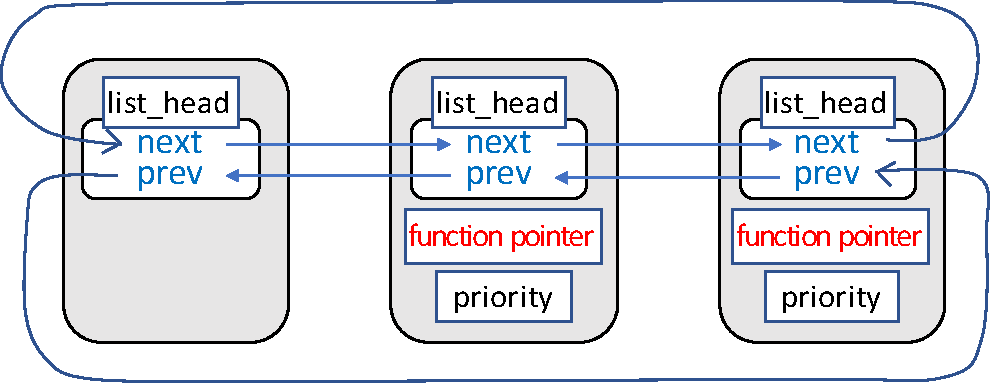
\includegraphics[width=90mm]{pics/dll.pdf}
	\caption{Structure of Doubly Linked List}
	\label{fig: dll}
\end{figure*}

\begin{figure*}
	\centering
	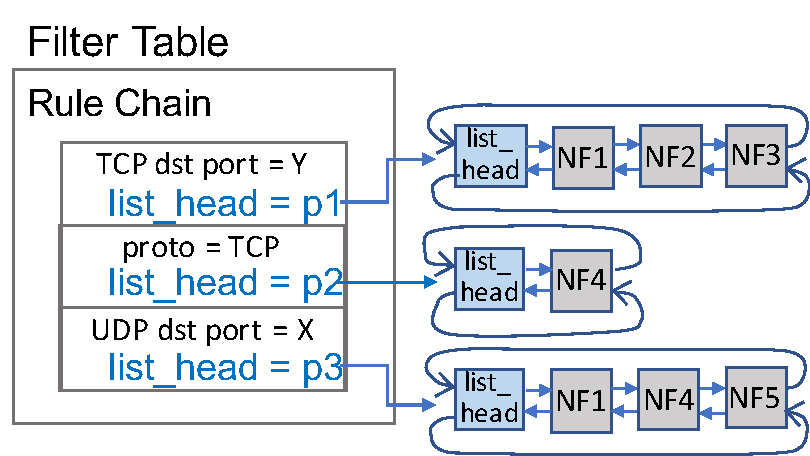
\includegraphics[width=90mm]{pics/list_head.pdf}
	\caption{list head}
	\label{fig: listhead}
\end{figure*}

 When inserting a NF in a chain, the priority and the function to be registered must be given. According to this information and network namespace, a nf\_target struct is created and inserted in the corresponding DLL. The struct is inserted before the node that has higher priority. 
 
 Figure \ref{fig: listhead} shows the example of Filter table and how the DLL that represents NF chain is linked. The mechanism that is responsible for NF chaining is called NFC system from here. When a packet arrives at the chaining point, it first traverse the Filter table to be passed to the right NF chaining. If a rule matches, the corresponding chaining starts: The NFC system takes the list head of the registered NF chain from the target component. Now from the next node in the DLL, which is the first NF, starts the process. The pointer to the SKB is passed to the the registered function in the node which will starts the entire the NF process. When the process is finished, the control comes back to the NFC system. At this point the function in the node returns verdict as well. There are only two types of them, DROP or ACCEPT. If it returns DROP, the NFC system stops the chaining and the SKB will be freed. Otherwise the system pass the SKB pointer to the function in the next node to process the next NF. The same procedure will continue until the last NF in the chain is executed. When the last NF returns ACCEPT, the NFC system ends NF chaining for the SKB and it will move to the next stage of network stack. 

As an example, when a UDP packet with destination port X arrives in the Filter table configured like \ref{fig: listhead}, the first and second NF chains are skipped. And the packet matches the last rule so the NF chaining of NF1, NF4 and NF5 starts. If all functions of NFs return ACCPET, this SKB that is probably modified by three NFs continues its journey in the network stack. 
